\documentclass[12pt,onecolumn,a4paper]{article}
\usepackage{epsfig,amsthm,amsmath,booktabs,csquotes}
\usepackage [pagebackref=true, colorlinks, linkcolor=blue, citecolor=magenta, urlcolor=cyan] {hyperref}
\usepackage{color,xcolor}

\usepackage{subcaption}
\usepackage[labelformat=parens,labelsep=quad, skip=3pt]{caption}
\usepackage{graphicx}
\usepackage{enumerate,braket}
\usepackage[localise]{xepersian}
%\settextfont[Scale=1.2]{‌BNAZANIN.TTF}
\settextfont[Scale=1.2]{BZAR.TTF}
\setlatintextfont[Scale=1]{Times New Roman}





\begin{document}
\title{سیر مطالعاتی من برای ارائه پایان نامه کارشناسی ارشد} 
\author{محسن مهرانی - استاد راهنما: دکتر سامان مقیمی عراقی}
\date{}
\maketitle
\قسمت{مطالعه مقاله شماره \cite{PhysRevLett.105.158104}:} 
در این مقاله مدلی را مشاهده کردیم که به کمک مدل $KM$ یک شبکه نورونی کامل را توصیف کرده است. این شبکه شامل نورون‌های مهاری است که روشن شدن هر کدوم از آن‌ها باعث مهار شدن نورون‌های همسایه می‌شود. معادله تحول اختلاف پتانسیل هر کدام از نورون‌ها با محیط بیرونش از رابطه زیر داده می‌شود ($g:$ ضریب اتصال هر جفت نورون، $S:$ ماتریس اتصال، $t_d$ زمان تاخیر میان زدن تیزه و تحریک آن، $a_i$ یک پتانسیل تحریکی و خارجی):
\begin{align}
\dot{v_i}=a_i - v_i - \frac{g}{N} \sum_{n|t_n<t} S_{i,l(n)} \delta(t - t_n - t_d) 
\label{eq:potential_1}
\end{align}

پارامتر نظم سیستم را به کمک میدان ($E$) تعریف کرده است اما پارامتر نظم را انحراف از معیار آن در طول زمان معرفی کرده است.
\begin{align}
\ddot{E}+ 2\alpha \dot{E}+\alpha^{2}E &=2\alpha N \sum_{n|tـn<t} \delta(t - t_n - t_d) \\
\sigma^{2} &= \braket{E^{2}}_{t} - \braket{E}^{2}_{t}
\end{align}
در طول زمان میدان $E$ و $\sigma$ را رصد کرده است و دیده‌است که میدان خاموش و روشن می‌شود و انحراف از معیار آن مقدار خوبی مثبت است چنان که این خاموش و روشن‌ها را با معنا نشان می‌دهد. حال ادعای این مقاله است که این خاموش و روشن شدن‌ها الگویی آشوبناک دارند و ادعا کرده است که به اندازه متناهی سامانه نیز وابسته نیست.\\

\subsection{سوالات}

\begin{enumerate}
\item
مدل $Kuramoto$ به قرار زیر است. چطور معادله \ref{eq:potential_1} به آن تبدیل می‌شود. دلتای یاد شده در معادله \ref{eq:potential_1} دلتای دیراک است؟ یا دلتایی که بیشینه آن عدد یک است؟ 
\begin{align}
\frac {d\theta _{i}}{dt}=\omega _{i}+\sum _{j=1}^{N}a_{ij}\sin(\theta _{j}-\theta _{i}),\qquad i=1\ldots N
\end{align}
\item
$t_n$ چیست؟
\item
اگر قرار باشد جمعی که در رابطه \ref{eq:potential_1} نوشته‌ایم روی تمام زمان‌های از ازل تا $t$ باشد پس آیا هر نورون حافظه‌ای از کل رخدادهای گذشته دارد؟ حتی از لحظاتی که قبل از تیزه زدن ها وجود دارند؟
\item
میدان $E$ به چه معناست؟ چطور تعریف کردیم؟ آیا مشخصه‌ای از کل سیستم است؟
\end{enumerate}

\textbf{پاسخ استاد:}
\begin{enumerate}
\item
قرار نیست کوراموتو به این تبدیل بشود. ممکنه یه شباهت‌های کلی‌ (به این معنی که مثلا دور می‌زنند) باشه ولی کلا دو تا معادله‌ی متفاوتند. در ضمن تابع دلتای دیراک است.
\item
کمیت‌های $t_n$ زمان‌هایی است که تیزه‌ای در سیستم زده می‌شود. [*می‌گویم: پس احتمالا معادله دیفرانسیلی ما دائم در حال به روز کردن سمت راست خودش است. هر وقت نورونی تیزه زد آن را در جمله سمت راست ذخیره می‌کنیم. پس احتمالا تقارن زمانی نداریم مگر پس مدتی طولانی که تاثیر شرایط اولیه بسیار کوچک دیده شود.]
\item
داستان اینه که هر نورونی که تیزه بزنه، اطرافیانش رو تحت تاثیر قرار می‌ده. پس وضعیت نورون به تمام تیزه‌های زمان‌های قبل وابسته است.
\item
هر وقت در هر جای دستگاه، تیزه‌ای زده بشه، کمیت$E$ کمی بالا می‌ره و بعد افت پیدا می‌کنه. حالا اگر تند و تند جا‌های مختلف تیزه زده بشه، این کمیت کم و بیش مقداری غیر صفر پیدا می‌کنه.[این کمیت را خودمون تعریف کرده‌ایم که بر حسب پارامترهای سیستم متحول می‌شود. مانند یک آشکارساز که به سامانه متصل می‌شود تا اندازه‌گیری خود را با یک عقربه نشان دهد.] اما اگر این تیزه زدن‌ها همگام باشه، یعنی همه با هم یه زمانی بزنند و بعد یه مدتی خاموش باشند، این کمیت، اول کلی زیاد می‌شه و بعد یه مدتی کم می‌مونه و در نتیجه انحراف معیارش زیاد می‌شه.
\end{enumerate}

\subsection{مسائل پیشروی پیاده سازی شبیه سازی}
\subsubsection{تابع بی‌کران دلتا}
یکی از مشکلات شبیه سازی معادلات دیفرانسیلی حضور تابع دلتای دیراک است. این تابع در نقطه صفر خود دارای مقداری بینهایت است. برای برطرف کردن این معذل چه باید کرد؟ نکته در این جا نهفته است که چون ما برای حل عددی معادله دیفرانسیلی خود از زمان پیوسته استفاده نمی‌کنیم و از گام‌هایی با طول مثبت $\Delta t$ استفاده می‌کنیم این مشکل به صورت زیر مدیریت می‌شود.
\begin{align}
v_{i}(t+\Delta t) &= v_{i}(t) + \int_{t}^{t+\Delta t} \dot{v_i}  dt \\
&= v_{i}(t) + \int_{t}^{t+\Delta t} \left[ a_i - v_i - \frac{g}{N} \sum_{n|t_n<t} S_{i,l(n)} \delta(t - t_n - t_d)  \right]   dt \\
&\approx v_{i}(t) +  \left[ a_i - v_i(t) \right] \Delta t - \frac{g}{N} \sum_{n|t_n<t} S_{i,l(n)} \int_{t}^{t+\Delta t} \delta(t - t_n - t_d) dt  \\
&\approx v_{i}(t) +  \left[ a_i - v_i(t) \right] \Delta t - \frac{g}{N} \sum_{n|t_n<t} S_{i,l(n)} H(t + \Delta t- t_n - t_d) \label{eq:potential_changes}
\end{align}

حالا تابع پله کاملا برای ما آشنا و قابل مدلسازی است. دقت شود که تابع پله یاد شده فقط در محدوده $t, t+\Delta t$ زندگی می‌کند و پس از آن اعتبار ندارد. معادله \ref{eq:potential_changes}  می‌گوید که باید برای تحول پتانسیل نورون $i$ام بررسی کنیم که آیا نورونی در همسایگی آن تیزه زده است یا نه. اگر چنان باشد یک واحد به جمع تیزه زدگان اضافه کنیم.


\subsubsection{ثبت تاریخ تیزه زدن‌ها}
برای محاسبه تحول پتانسیل در رابطه \ref{eq:potential_changes} چنان که توضیح داده شد نیاز به دانستن تاریخ تیزه زدن‌ها هستیم. در صورت ثبت زمان تیزه زدن برای هر نورون، یک آرایه مربعی خواهیم داشت که شماره سطر آن می‌تواند معرف زمان باشد و ستون نماد شماره نورون. شکل شماره (\ref{fig:rasterplot})
\begin{figure}
\centering
  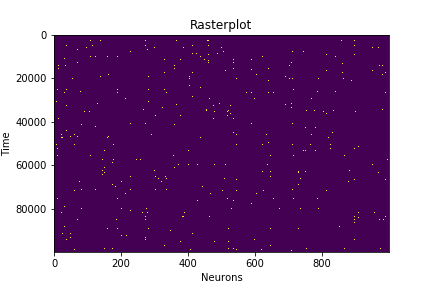
\includegraphics[width = 10 cm]{../scripts/kuramoto_model_synchoronization_problem/raster_plot_N1000.png}
 \caption{ثبت لحظه‌ای تیزه زدن هر نورون به صورت مجزا - در این نمودار ضریب تاثیر هر نورون روی همسایه‌هایش $g = 5$ بوده است. چنان که انتظار می‌رفت شاهد هم‌گامی هستیم.}
  \label{fig:rasterplot}
\end{figure}
اما مشکلی که برای این شبیه سازی رخ خواهد داد آن است که در صورت افزایش تعداد نورون‌ها و زمان شبیه سازی با یک ابر آرایه روبرو خواهیم شد که امکان دارد در ذخیره سازی آن دچار مشکل شویم. به همین خاطر در شبیه سازی انجام شده تنها مجموع تیزه زدن‌ها را ذخیره کردیم تا یک آرایه یک ستونه داشته باشیم و در ذخیره‌سازی به مشکل نخوریم.

\subsection{نتایج}
در این قسمت به خروجی شبیه سازی می‌پردازیم. این شبیه سازی برای ۱۰۰۰ ثانیه اجرا شده است که در آن هر گام زمانی برابر ۰.۰۱ ثانیه گرفته شده است. بقیه پارامترها هم کاملا از صورت مقاله برداشته شده اند. کد شبیه‌سازی در پوشه 
\href{run://..//scripts//kuramoto_model_synchoronization_problem}{مسئله همگامی برای مدل کوراموتو}
قابل مشاهده است.\\
مهم‌ترین شاخصه ما برای ردگیری همگامی، انحراف معیار $E$ است که با زیگما $\sigma$ نمایش می‌دهیم. جهش به وجود آمده در شکل‌ (\ref{fig:two_pops_sync}) به این معنی است که سامانه از حالت ناهم‌گامی به هم‌گامی تغییر فاز داده است. نکته قابل توجه آن است که با افزایش تعداد نورون‌ها این دو فاز از یک دیگر متمایزتر می‌شوند و فاصله‌ی رفتاری آن‌ها بیشتر می‌شود.

\begin{figure}
\centering
  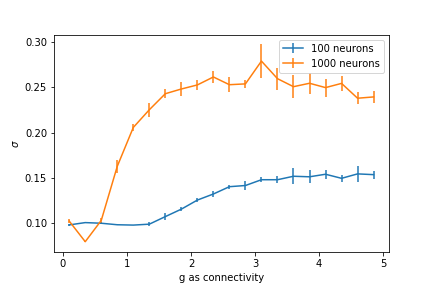
\includegraphics[width = 10 cm]{../scripts/kuramoto_model_synchoronization_problem/two_pops_sigma.png}
 \caption{تغییر فاز از ناهم‌گامی به هم‌گامی برای دو جمعیت متفاوت}
  \label{fig:two_pops_sync}
\end{figure}

\section{شبیه‌سازی مدل چرخنده}
در این مدل به جای آن که برای شبکه خود از مدل انباشت-شلیک استفاده کنیم از مدل چرخنده استفاده می‌کنیم. این مدل نسبت به مدل قبلی شامل ویژگی‌های مثبتی است. یکی از ویژگی‌های خوب آن این است که برای قسمت شلیک یک منحنی پیوسته ارائه می‌کند و دیگر پتانسیل آن نیازی به بازنشانی لحظه‌ای ندارد. برای توصیف فاز هر نورون از معادلات زیر استفاده می‌کنیم:
\begin{equation}
\begin{cases}
\dot{\theta_i}=I_i - cos(\theta_i) - g E \\
\dot{E} = M - \alpha E\\
\dot{M} = -  \alpha M + \frac{ \alpha^{2} }{N} \sum_{n|tـn<t} \delta(t - t_n - t_d)
\end{cases}
\end{equation}
برای تشخیص هم‌گامی ما شاخصه نظمی را مطابق زیر تعریف کردیم:
\begin{equation}
s = \frac{1}{N} \sum_{i} sin^{2}(\theta_i)
\end{equation}

\subsection{شبیه‌سازی}
حال می‌خواهیم که شبکه کامل شامل این نورون‌ها را مدلسازی کنیم تا مجددا بپرسیم آیا تغییر در قدرت اتصال $g$ می‌تواند باعث شود تا تغییر فاز از ناهم‌گامی به هم‌گامی رخ دهد؟ برای مشاهده دفترچه شبیه‌سازی به آدرس 
\href{run://..//scripts//rotational_model}{مسئله همگامی برای مدل چرخنده}
مراجعه کنید.
\subsubsection{مشکل: شاخصه نظم}
مهم‌ترین علاقه‌مندی ما هم‌گام شدن نورون‌ها هستند. یعنی اگر همگی در یک فاز همراه هم باشند هم‌گامی کامل داریم. اما شاخصه نظم ما اعداد متفاوتی را نشان خواهد اگر همگی در ابتدای ربع دوم باشند یا همگی در انتهای آن. پس شاید بهتر باشد شاخصه نظم خود را تغییر دهیم.
\subsubsection{مشکل: به پیمانه گرفتن}
در معادلات برای ما مهم است که تنها روابط هندسی فاز هر نورون را بدانیم. حال برای آن که هم‌فازها را تشخیص دهیم می‌توانیم فاز‌های خارج از دایره‌ی صفر تا $2\pi$ را به آن مجددا بازرسانیم. اما جالب است اگر این تغییر را درمیانه حلقه شبیه‌سازی انجام دهیم آمار فاز نورون‌ها نیز تغییر می‌کند. در حالتی که $g=0$ است انتظار داریم تا همگی در فاز‌های متفاوتی به صورت یکنواخت توزیع شده باشند اما با به پیمانه زدن این اتفاق نمی‌افتد و حول صفر و $2\pi$ انباشتگی ملاحظه می‌شود.

\subsubsection{مشکل: یک تیزه را چند بار می‌شماریم؟}
برای آن که علامت بزنیم که کدام نورون تیزه زده است، می‌توانیم یک بازه‌ی خاص را حول $\pi$ در نظر بگیریم و هر گاه فاز نورون از آن بازه رد شد به عنوان تیزه آن را حساب کنیم. اما یک مشکل فرآیندی در شبیه‌سازی به وجود می‌آید که چگونه متوجه شویم که فاز نورونی از روی آن بازه نپریده است. هر گام زمانی ما می‌تواند لحظاتی گسسته را از حالت نورون رصد کند. پس این مشکل محتمل است و باید برای فرآیند شماره تیزه چاره‌ای بیندیشیم.
\subsubsection{}
\subsection{}


\newpage
\bibliographystyle{plain-fa}
\bibliography{MyReferences}

\end{document}


